% Author: Cyrille Chenavier, Christophe Cordero, Samuele Giraudo
% Creation: may. 2018
% Modifications: may. 2018, june 2018

\documentclass[10pt,reqno]{amsart}

%%%%%%%%%%%%%%%%%%%%%%%%%%%%%%%%%%%%%%%%%%%%%%%%%%%%%%%%%%%%%%%%%%%%%%%%
%%%%%%%%%%%%%%%%%%%%%%%%%%%%%%%%%%%%%%%%%%%%%%%%%%%%%%%%%%%%%%%%%%%%%%%%
%%%%%%%%%%%%%%%%%%%%%%%%%%%%%%%%%%%%%%%%%%%%%%%%%%%%%%%%%%%%%%%%%%%%%%%%
\usepackage[utf8x]{inputenc}
\usepackage[english]{babel}
\usepackage{amsmath,amsfonts,amssymb,amsthm,shuffle}
\usepackage[T1]{fontenc}
\usepackage[math]{anttor}

% Layout.
\usepackage[top=3.5cm,bottom=3.5cm,left=3.6cm,right=3.6cm]{geometry}

% Colors of hyperlinks.
\usepackage{xcolor}
% Author: Samuele Giraudo
% Creation: mar. 2018
% Modifications: mar. 2018

\definecolor{ColBlack}{RGB}{0,0,0} % Black.
\definecolor{ColWhite}{RGB}{255,255,255} % White.
\definecolor{Col1}{RGB}{133,6,6} % Rouge sang.
\definecolor{Col2}{RGB}{198,8,0} % Rouge ponceau.
\definecolor{Col3}{RGB}{174,74,52} % Rouge tomette.
\definecolor{Col4}{RGB}{103,113,121} % Gris de Payne.
\definecolor{Col5}{RGB}{90,94,107} % Ardoise.
\definecolor{Col6}{RGB}{70,63,50} % Taupe.

\newcommand{\ColBlack}[1]{\textcolor{ColBlack}{#1}}
\newcommand{\ColWhite}[1]{\textcolor{ColWhite}{#1}}
\newcommand{\ColA}[1]{\textcolor{Col1}{#1}}
\newcommand{\ColB}[1]{\textcolor{Col2}{#1}}
\newcommand{\ColC}[1]{\textcolor{Col3}{#1}}
\newcommand{\ColD}[1]{\textcolor{Col4}{#1}}
\newcommand{\ColE}[1]{\textcolor{Col5}{#1}}
\newcommand{\ColF}[1]{\textcolor{Col6}{#1}}


\usepackage[hyperindex=true,frenchlinks=true,colorlinks=true,
citecolor=Col2,linkcolor=Col3,urlcolor=Col4,linktocpage,
pagebackref=true]{hyperref}

% Tikz.
\usepackage{tikz}
\usetikzlibrary{shapes}
\usetikzlibrary{fit}
\usetikzlibrary{decorations.pathmorphing}

% Misc.
\usepackage{mathtools}
\usepackage{dsfont}
\usepackage{wasysym}
\usepackage{stmaryrd}
\usepackage{cite}
\usepackage{subfig}
\usepackage{multirow}
\usepackage{enumitem}
\usepackage{multicol}
\usepackage{cancel}

%%%%%%%%%%%%%%%%%%%%%%%%%%%%%%%%%%%%%%%%%%%%%%%%%%%%%%%%%%%%%%%%%%%%%%%%
%%%%%%%%%%%%%%%%%%%%%%%%%%%%%%%%%%%%%%%%%%%%%%%%%%%%%%%%%%%%%%%%%%%%%%%%
%%%%%%%%%%%%%%%%%%%%%%%%%%%%%%%%%%%%%%%%%%%%%%%%%%%%%%%%%%%%%%%%%%%%%%%%
% Line space.
\linespread{1.15}
\renewcommand{\arraystretch}{1.4}

% Vertical space for equations.
\setlength{\abovedisplayskip}{5pt}
\setlength{\belowdisplayskip}{5pt}

% Alphabetic footnote marks.
\renewcommand{\thefootnote}{\alph{footnote}}

% To allow cutting equations in several pages.
\allowdisplaybreaks

% Numbering of equations.
\numberwithin{equation}{subsection}

% Depth of the table of contents.
\setcounter{tocdepth}{2}

% Indentation in the table of contents.
\makeatletter
\def\l@section{\@tocline{1}{3pt}{1pc}{5pc}{}}
\def\l@subsection{\@tocline{2}{2pt}{2pc}{5pc}{}}
\makeatother

% Environments definitions.
\newtheorem{Theorem}{Theorem}[subsection]
\newtheorem{Proposition}[Theorem]{Proposition}
\newtheorem{Lemma}[Theorem]{Lemma}

% Better comparison symbols.
\renewcommand{\leq}{\leqslant}
\renewcommand{\geq}{\geqslant}

%%%%%%%%%%%%%%%%%%%%%%%%%%%%%%%%%%%%%%%%%%%%%%%%%%%%%%%%%%%%%%%%%%%%%%%%
%%%%%%%%%%%%%%%%%%%%%%%%%%%%%%%%%%%%%%%%%%%%%%%%%%%%%%%%%%%%%%%%%%%%%%%%
%%%%%%%%%%%%%%%%%%%%%%%%%%%%%%%%%%%%%%%%%%%%%%%%%%%%%%%%%%%%%%%%%%%%%%%%
\title{Comb associative operads}
\keywords{Operad; trees; Rewrite rule; Presentation; Enumeration.}
\subjclass[2010]{\Todo{}}
\date{\today}
\author{Cyrille Chenavier \and Christophe Cordero \and Samuele Giraudo}
\address{\scriptsize Université Paris-Est, LIGM (UMR $8049$), CNRS,
    ENPC, ESIEE Paris, UPEM, F-$77454$, Marne-la-Vallée, France}
\email{cyrille.chenavier@u-pem.fr}
\email{christophe.cordero@u-pem.fr}
\email{samuele.giraudo@u-pem.fr}

%%%%%%%%%%%%%%%%%%%%%%%%%%%%%%%%%%%%%%%%%%%%%%%%%%%%%%%%%%%%%%%%%%%%%%%%
%%%%%%%%%%%%%%%%%%%%%%%%%%%%%%%%%%%%%%%%%%%%%%%%%%%%%%%%%%%%%%%%%%%%%%%%
%%%%%%%%%%%%%%%%%%%%%%%%%%%%%%%%%%%%%%%%%%%%%%%%%%%%%%%%%%%%%%%%%%%%%%%%
% Author: Samuele Giraudo
% Creation: mar. 2018
% Modifications: mar. 2018

% Tools macros.
\newcommand{\Todo}[1]{\textcolor{Col1}{{\tt TODO: $[$#1$]$}}}
\newcommand{\Hide}[1]{\textcolor{Col4}{\tt [hidden]}}

% Format macros.
\newcommand{\Def}[1]{\textcolor{Col3}{\em #1}}
\newcommand{\OEIS}[1]{\href{http://oeis.org/#1}{{\bf #1}}}
\newcommand{\Arxiv}[1]{\href{https://arxiv.org/abs/#1}{\tt arXiv:#1}}

% Tikz for vertical centering.
\tikzstyle{Centering}=[{baseline={([yshift=-0.5ex]current
    bounding box.center)}}]


\newcommand{\N}{\mathbb{N}}
\newcommand{\Z}{\mathbb{Z}}
\newcommand{\Q}{\mathbb{Q}}
\newcommand{\K}{\mathbb{K}}

\newcommand{\Oca}{\mathcal{O}}
\newcommand{\Rfr}{\mathfrak{r}}
\newcommand{\Sfr}{\mathfrak{s}}
\newcommand{\Tfr}{\mathfrak{t}}

\newcommand{\Zero}{\mathtt{0}}
\newcommand{\Two}{\mathtt{2}}
\newcommand{\HilbertSeries}{\mathcal{H}}
\newcommand{\GeneratingSet}{\mathfrak{G}}
\newcommand{\FreeOperad}{\mathrm{F}}
\newcommand{\Mag}{\mathsf{Mag}}
\newcommand{\As}{\mathsf{As}}
\newcommand{\CAs}[1]{\mathsf{CAs}^{(#1)}}
\newcommand{\CAsAll}{\mathbf{CAs}}
\newcommand{\PrefixWord}{\mathrm{p}}
\newcommand{\Deg}{\mathrm{deg}}
\newcommand{\LComb}[1]{\mathfrak{c}^{(#1)}_{\diagup}}
\newcommand{\RComb}[1]{\mathfrak{c}^{(#1)}_{\diagdown}}
\newcommand{\LBranch}{\mathrm{lb}}
\newcommand{\RBranch}{\mathrm{rb}}
\newcommand{\Catalan}{\mathrm{cat}}
\newcommand{\OrdCAs}{\preceq}

\DeclareMathOperator{\Product}{\star}
\DeclareMathOperator{\Congr}{\equiv}
\DeclareMathOperator{\Rew}{\to}
\DeclareMathOperator{\RewRT}{\overset{*}{\Rew}}
\DeclareMathOperator{\RewT}{\overset{+}{\Rew}}
\DeclareMathOperator{\RewRTS}{\overset{*}{\leftrightarrow}}
\DeclareMathOperator{\RewContext}{\Rightarrow}
\DeclareMathOperator{\RewContextRT}{\overset{*}{\RewContext}}
\DeclareMathOperator{\RewContextT}{\overset{+}{\RewContext}}
\DeclareMathOperator{\lcm}{lcm}

\newcommand{\CongrCAs}[1]{\Congr^{(#1)}}

% Tree drawings.
\tikzstyle{Node}=[circle,draw=Col1!80,fill=Col1!8,inner sep=1pt,
minimum size=2mm,thick,font=\scriptsize]
\tikzstyle{Edge}=[draw=Col2!80,cap=round,thick]
\tikzstyle{Leaf}=[rectangle,draw=ColBlack!70,fill=ColBlack!16,
inner sep=0pt,minimum size=1mm,thick]
\tikzstyle{NodeST}=[font=\footnotesize]

%%%%%%%%%%%%%%%%%%%%%%%%%%%%%%%%%%%%%%%%%%%%%%%%%%%%%%%%%%%%%%%%%%%%%%%%
%%%%%%%%%%%%%%%%%%%%%%%%%%%%%%%%%%%%%%%%%%%%%%%%%%%%%%%%%%%%%%%%%%%%%%%%
%%%%%%%%%%%%%%%%%%%%%%%%%%%%%%%%%%%%%%%%%%%%%%%%%%%%%%%%%%%%%%%%%%%%%%%%
\begin{document}

%%%%%%%%%%%%%%%%%%%%%%%%%%%%%%%%%%%%%%%%%%%%%%%%%%%%%%%%%%%%%%%%%%%%%%%%
%%%%%%%%%%%%%%%%%%%%%%%%%%%%%%%%%%%%%%%%%%%%%%%%%%%%%%%%%%%%%%%%%%%%%%%%
%%%%%%%%%%%%%%%%%%%%%%%%%%%%%%%%%%%%%%%%%%%%%%%%%%%%%%%%%%%%%%%%%%%%%%%%
\begin{abstract}
    The associative operad is the quotient of the magmatic operad by
    the operad congruence identifying the two binary trees of degree
    $2$. We introduce here a generalization of the associative operad
    depending on a nonnegative integer $d$, called $d$-comb associative
    operad, as the quotient of the magmatic operad by the operad
    congruence identifying the left and the right comb binary trees of
    degree $d$. We study the case $d = 3$ and provide an orientation
    of its space of relations by using rewrite systems on trees and
    the Buchberger algorithm for operads to obtain a convergent
    rewrite system.
\end{abstract}

\maketitle

\tableofcontents

%%%%%%%%%%%%%%%%%%%%%%%%%%%%%%%%%%%%%%%%%%%%%%%%%%%%%%%%%%%%%%%%%%%%%%%%
%%%%%%%%%%%%%%%%%%%%%%%%%%%%%%%%%%%%%%%%%%%%%%%%%%%%%%%%%%%%%%%%%%%%%%%%
%%%%%%%%%%%%%%%%%%%%%%%%%%%%%%%%%%%%%%%%%%%%%%%%%%%%%%%%%%%%%%%%%%%%%%%%
\section*{Introduction}
Associative algebras are spaces endowed with a binary product $\Product$
satisfying among others the associativity law
\begin{math}
    (x_1 \Product x_2) \Product x_3 = x_1 \Product (x_2 \Product x_3)
\end{math}.
It is well-known that the associative algebras are representations of
the associative (nonsymmetric) operad $\As$. This operad can be seen as
the quotient of the magmatic operad $\Mag$ (the free operad of binary
trees on the binary generator~$\Product$) by the operad congruence
$\Congr$ satisfying
\begin{equation} \label{equ:congruence_as}
    \begin{tikzpicture}[xscale=.24,yscale=.24,Centering]
        \node(0)at(0.00,-3.33){};
        \node(2)at(2.00,-3.33){};
        \node(4)at(4.00,-1.67){};
        \node[NodeST](1)at(1.00,-1.67)
            {\begin{math}\Product\end{math}};
        \node[NodeST](3)at(3.00,0.00)
            {\begin{math}\Product\end{math}};
        \draw[Edge](0)--(1);
        \draw[Edge](1)--(3);
        \draw[Edge](2)--(1);
        \draw[Edge](4)--(3);
        \node(r)at(3.00,1.5){};
        \draw[Edge](r)--(3);
    \end{tikzpicture}
    \Congr
    \begin{tikzpicture}[xscale=.24,yscale=.24,Centering]
        \node(0)at(0.00,-1.67){};
        \node(2)at(2.00,-3.33){};
        \node(4)at(4.00,-3.33){};
        \node[NodeST](1)at(1.00,0.00)
                {\begin{math}\Product\end{math}};
        \node[NodeST](3)at(3.00,-1.67)
                {\begin{math}\Product\end{math}};
        \draw[Edge](0)--(1);
        \draw[Edge](2)--(3);
        \draw[Edge](3)--(1);
        \draw[Edge](4)--(3);
        \node(r)at(1.00,1.5){};
        \draw[Edge](r)--(1);
    \end{tikzpicture}\,.
\end{equation}
These two binary trees are the syntax trees of the expressions appearing
in the above associativity law.
\medbreak

In a more combinatorial context and regardless of the theory of operads,
the Tamari order is a partial order on the set of the binary trees
having a fixed number of internal nodes $d$. This order is generated by
the covering relation consisting in rewriting a tree $\Tfr$ into a tree
$\Tfr'$ by replacing a subtree of $\Tfr$ of the form of the left member
of~\eqref{equ:congruence_as} into a tree of the form of the right member
of~\eqref{equ:congruence_as}. This transformation is known in a computer
science context as the right rotation operation~\cite{Knu98} and
intervenes in algorithms involving binary search trees~\cite{AVL62}. The
partial order hence generated by the right rotation operation is known
as the Tamari order~\cite{Tam62} and has a lot of combinatorial and
algebraic properties (see for instance~\cite{HT72,Cha06}).
\medbreak

A first connection between the associative operad and the Tamari order
is based upon the fact that the orientation of~\eqref{equ:congruence_as}
from left to right provides a convergent orientation (a terminating and
confluent rewrite relation) of the congruence $\Congr$. The normal
forms of the rewrite relation induced by the rewrite rule obtained by
orienting~\eqref{equ:congruence_as} from left to right are right comb
binary trees and are hence in one-to-one correspondence with the
elements of~$\As$.
\medbreak

This work is intended to be a first strike in the study of the eventual
links between the Tamari order and some quotients of the operad $\Mag$.
In the long run, we would like to study quotients $\Mag/_{\Congr}$ of
$\Mag$ where $\Congr$ is an operad congruence generated by equivalence
classes of trees of a fixed degree. In particular, we would like to know
if $\Congr$ is generated by equivalence classes of trees forming
intervals of the Tamari order leads to algebraic properties for
$\Mag/_{\Congr}$ (like the description of orientations of its space of
relations, nice bases and Hilbert series).
\medbreak

We focus here on one of these quotients $\CAs{3}$ which is the operad
describing the category of the algebras equipped with a binary product
$\Product$ and subjected to the relation
\begin{math}
    ((x_1 \Product x_2) \Product x_3) \Product x_4
    =
    x_1 \Product (x_2 \Product (x_3 \Product x_4))
\end{math}.
This is a kind of associativity law in higher degree $d = 3$. This
operad is generated by an equivalence class of trees which is not an
interval for the Tamari order. As preliminary computer experiments show,
$\CAs{3}$ has oscillating first dimensions
(see~\eqref{equ:dimensions_CAs_3}), what is rather unusual among all
known operads. In this paper, we provide an orientation of the space of
relations of $\CAs{3}$. For this, we use rewrite systems on
trees~\cite{BN98} and the Buchberger algorithm for operads~\cite{DK10}.
\medbreak

This text is presented as follows. Section~\ref{sec:operad_Mag} contains
preliminaries about the magmatic operad and rewrite relations on trees.
In Section~\ref{sec:CAs_d}, we define the operad $\CAs{3}$ as a
particular case of a more general construction of generalizations
$\CAs{d}$, $d \geq 1$, of $\As$. Finally, Section~\ref{sec:CAs_3}
contains the orientation of the space of relations of
$\CAs{3}$ (Theorem~\ref{thm:convergent_rewrite_rule_CAs_3}). As
consequences, we obtain for $\CAs{3}$
the description of one of its Poincaré-Birkhoff-Witt bases
(Proposition~\ref{prop:PBW_basis_CAs_3}) and the description of
its Hilbert series (Proposition~\ref{prop:Hilbert_series_CAs_3}).
\medbreak

%%%%%%%%%%%%%%%%%%%%%%%%%%%%%%%%%%%%%%%%%%%%%%%%%%%%%%%%%%%%%%%%%%%%%%%%
%%%%%%%%%%%%%%%%%%%%%%%%%%%%%%%%%%%%%%%%%%%%%%%%%%%%%%%%%%%%%%%%%%%%%%%%
%%%%%%%%%%%%%%%%%%%%%%%%%%%%%%%%%%%%%%%%%%%%%%%%%%%%%%%%%%%%%%%%%%%%%%%%
\section{The magmatic operad, quotients, and rewrite relations}
\label{sec:operad_Mag}
We consider nonsymmetric set-theoretic operads. Let $\Oca$ be such an
operad. We denote respectively by $\circ_i$ and $\circ$ the partial and
complete compositions of $\Oca$. For any $n \geq 1$, $\Oca(n)$ is the
set of the elements $x$ of $\Oca$ of arity $|x| = n$. We denote
by $\Mag$ the magmatic operad, that is the free operad over one binary
generator $\Product$, and we represent the elements of $\Mag$ by binary
trees. The \Def{arity} $|\Tfr|$ (resp. \Def{degree} $\Deg(\Tfr)$) of a
binary tree $\Tfr$ is its number of leaves (resp. internal nodes).
Recall that for any positive integer $n$,
$\# \Mag(n)$ is the $n$th Catalan number
$\Catalan(n) := \binom{2n - 2}{n - 1}\frac{1}{n}$.
\medbreak

Given a binary tree $\Tfr$, we denote by $ \PrefixWord(\Tfr)$ the
\Def{prefix word} of $\Tfr$, that is the word on $\{\Zero, \Two\}$
obtained by a left to right depth-first traversal of $\Tfr$ and by
writing $\Zero$ (resp. $\Two$) when a leaf (resp. an internal node) is
encountered. The set of all words on $\{\Zero, \Two\}$ is endowed with
the lexicographic order $\leq$ induced by $\Zero < \Two$.
\medbreak

If $\Rew$ is a rewrite rule on $\Mag$ such that $\Sfr \Rew \Sfr'$
implies $|\Sfr| = |\Sfr'|$, we denote by $\RewContext$ the
\Def{rewrite relation induced} by $\Rew$. Formally we have
\begin{math}
    \Tfr\circ_i\left(\Sfr\circ\left[\Rfr_1,\dots,\Rfr_{n}\right]\right)
    \RewContext
    \Tfr\circ_i\left(\Sfr'\circ\left[\Rfr_1,\dots,\Rfr_{n}\right]\right)
\end{math},
if $\Sfr \Rew \Sfr'$ where $n = |\Sfr|$, and $\Tfr$, $\Rfr_1$, \dots,
$\Rfr_n$ are binary trees. In other words, one has
$\Tfr \RewContext \Tfr'$ if it is possible to obtain $\Tfr'$ from $\Tfr$
by replacing a subtree $\Sfr$ of $\Tfr$ by $\Sfr'$ whenever
$\Sfr \Rew \Sfr'$. We use here the standard terminology
(\Def{terminating}, \Def{confluent}, \Def{convergent}, \Def{branching
pair}, \Def{joinable}, \Def{normal form}, {\em etc.}) about rewrite
relations and rewrite systems~\cite{BN98}.
\medbreak

Given an operad $\Oca \simeq \Mag/_{\Congr}$ where $\Congr$ is an operad
congruence of $\Mag$, we denote by $[\Tfr]_{\Congr}$ the
$\Congr$-equivalence class of any $\Tfr \in \Mag$. Besides, we say that
$\Rew$ is an \Def{orientation} of $\Congr$ if the reflexive, transitive,
and symmetric closure of $\RewContext$ is $\Congr$. We say that $\Rew$
is a \Def{convergent orientation} if $\RewContext$ is convergent. When
$\Rew$ is a convergent orientation of $\Congr$, the set of all normal
forms of $\RewContext$ is a \Def{Poincaré-Birkhoff-Witt basis} of the
operad $\Oca$ and its elements are exactly the binary trees avoiding,
as subtrees, the trees appearing as left members in~$\Rew$.
\medbreak

We shall use the following criterion to prove that a rewrite relation on
$\Mag$ is terminating.
\medbreak

\begin{Lemma}\label{lem:prefix_word_termination}
    Let $\Rew$ be a rewrite rule on $\Mag$. If for any
    $\Tfr, \Tfr' \in \Mag$ such that $\Tfr \Rew \Tfr'$ one has
    $\PrefixWord(\Tfr) > \PrefixWord(\Tfr')$, then the rewrite relation
    induced by $\Rew$ is terminating.
\end{Lemma}
\medbreak

Moreover, we shall use the following result appearing in~\cite{Gir16}
specialized on rewrite relation on $\Mag$ to prove that a terminating
rewrite relation is convergent.
\medbreak

\begin{Lemma} \label{lem:degree_confluence}
    Let $\Rew$ be a rewrite rule on $\Mag$ wherein all trees $\Tfr$ and
    $\Tfr'$ such that $\Tfr \Rew \Tfr'$ have degrees at most $\ell$.
    Then, if the rewrite relation $\RewContext$ induced by $\Rew$ is
    terminating and all its branching pairs of degrees at most
    $2\ell - 1$ are joinable, $\RewContext$ is convergent.
\end{Lemma}
\medbreak

%%%%%%%%%%%%%%%%%%%%%%%%%%%%%%%%%%%%%%%%%%%%%%%%%%%%%%%%%%%%%%%%%%%%%%%%
%%%%%%%%%%%%%%%%%%%%%%%%%%%%%%%%%%%%%%%%%%%%%%%%%%%%%%%%%%%%%%%%%%%%%%%%
%%%%%%%%%%%%%%%%%%%%%%%%%%%%%%%%%%%%%%%%%%%%%%%%%%%%%%%%%%%%%%%%%%%%%%%%
\section{Generalizations of the associative operad} \label{sec:CAs_d}
\Todo{Write mini intro.}

%%%%%%%%%%%%%%%%%%%%%%%%%%%%%%%%%%%%%%%%%%%%%%%%%%%%%%%%%%%%%%%%%%%%%%%%
%%%%%%%%%%%%%%%%%%%%%%%%%%%%%%%%%%%%%%%%%%%%%%%%%%%%%%%%%%%%%%%%%%%%%%%%
\subsection{Comb associative operads}
\Todo{Write mini intro.}

It is known that the rewrite rule $\Rew$
orienting~\eqref{equ:congruence_as} from left to right is a convergent
orientation of (\ref{equ:congruence_as}). Then, a Poincaré-Birkhoff-Witt
basis of $\As$ is the set of all right comb binary trees.
\Todo{SG: to maybe to move at another place. }
\medbreak

Let, for any $\gamma \geq 1$, the binary trees
\begin{equation}
    \LComb{\gamma} :=
    \underbrace{(\dots (\Product \circ_1 \Product) \circ_1 \dots)
        \circ_1 \Product}
    _{\gamma \mbox{ \footnotesize operands}}
\end{equation}
and
\begin{equation}
    \RComb{\gamma} :=
    \underbrace{\Product \circ_2
        (\dots \circ_2 (\Product \circ_2 \Product) \dots)}
    _{\gamma \mbox{ \footnotesize operands}}
\end{equation}
be respectively the left and the right comb of degree $\gamma$.
Let us now define for any $\gamma \geq 1$ the \Def{$\gamma$-comb
associative operad} $\CAs{\gamma}$ as the quotient operad
$\Mag/_{\CongrCAs{\gamma}}$ where $\CongrCAs{\gamma}$ is the smallest
operad congruence of $\Mag$ satisfying
\begin{equation} \label{equ:congruence_CAs_gamma}
    \LComb{\gamma} \enspace \CongrCAs{\gamma} \enspace \RComb{\gamma}
\end{equation}
Notice that $\CongrCAs{1}$ is trivial so that
$\CAs{1} = \Mag$ and that $\CongrCAs{2}$ is the operad congruence
defined by~\eqref{equ:congruence_as} so that $\CAs{2} = \As$.
Let also
\begin{equation}
    \CAsAll := \left\{\CAs{\gamma} : \gamma\geq 1\right\}
\end{equation}
be the set of all the $\gamma$-comb associative operads
Our purpose is to show that $\CAsAll$ admits a lattice structure. For
that, we provide a description of operads morphisms between the
elements of~$\CAsAll$.
\medbreak

%%%%%%%%%%%%%%%%%%%%%%%%%%%%%%%%%%%%%%%%%%%%%%%%%%%%%%%%%%%%%%%%%%%%%%%%
%%%%%%%%%%%%%%%%%%%%%%%%%%%%%%%%%%%%%%%%%%%%%%%%%%%%%%%%%%%%%%%%%%%%%%%%
\subsection{A lattice of operads}
\Todo{Write mini intro.}

\begin{Lemma} \label{lem:first_dimensions_CAs}
    For any positive integers $\gamma$ and $n$ such that $\gamma \geq 2$
    and $n \leq \gamma + 1$,
    \begin{equation}
        \# \CAs{\gamma}(n) =
        \begin{cases}
            \Catalan(n)
                & \mbox{ if } n \leq \gamma, \\
            \Catalan(\gamma + 1) - 1
                & \mbox{ otherwise } (n = \gamma + 1).
        \end{cases}
    \end{equation}
\end{Lemma}
\begin{proof}
    Since the equivalence relation $\CongrCAs{\gamma}$ is trivial on the
    binary trees of degrees $d < \gamma$, and since a binary tree of
    degree $d$ has arity $n := d + 1$, one has
    $\# \CAs{\gamma}(n) = \# \Mag(n) = \Catalan(n)$ with $n \leq \gamma$.
    Besides, by definition of $\CongrCAs{\gamma}$, all the
    $\CongrCAs{\gamma}$-equivalence classes of binary trees of degree
    $\gamma$ are trivial, except one consisting in the pair
    $\left\{\LComb{\gamma}, \RComb{\gamma}\right\}$. Therefore, since a
    binary tree of degree $d$ has arity $n := \gamma + 1$,
    \begin{math}
        \# \CAs{\gamma}(n)
        = \# \Mag(\gamma + 1) - 1
        = \Catalan(\gamma + 1) - 1.
    \end{math}
\end{proof}
\medbreak

\begin{Lemma} \label{lem:surjective_morphisms_CAs}
    Let $\gamma$ and $\gamma'$ be two positive integers. If
    $\varphi:\CAs{\gamma'} \to \CAs{\gamma}$ is an operad morphism, then
    it is surjective and is unique.
\end{Lemma}
\begin{proof}
    The operad $\CAs{\gamma'}$ is generated by one binary generator
    $[\Product]_{\CongrCAs{\gamma'}}$, so that $\varphi$ is entirely
    determined by the image
    $\varphi\left([\Product]_{\CongrCAs{\gamma'}}\right)$. Moreover,
    $\varphi([\Product]_{\CongrCAs{\gamma'}})$ has to be of arity $2$ in
    $\CAs{\gamma}$, so that we necessarily have
    \begin{math}
        \varphi\left([\Product]_{\CongrCAs{\gamma'}}\right)
        =
        [\Product]_{\CongrCAs{\gamma}}.
    \end{math}
    Hence, if $\varphi$ exists, it is the unique operad morphism from
    $\CAs{\gamma'}$ to $\CAs{\gamma}$. In this case,
    $[\Product]_{\CongrCAs{\gamma'}}$ being in the image of $\varphi$,
    the latter is surjective.
\end{proof}
\medbreak

\begin{Lemma} \label{lem:injective_morphisms_CAs}
    Let $\gamma$ and $\gamma'$ be two positive integers and
    $\varphi:\CAs{\gamma'} \to \CAs{\gamma}$ be an operad morphism.
    Then, $\varphi$ is injective if and only if $\gamma = \gamma'$.
\end{Lemma}
\begin{proof}
    Assume that $\varphi$ is injective. By
    Lemma~\ref{lem:surjective_morphisms_CAs}, $\varphi$ is also
    surjective, so that $\varphi$ is an isomorphism. If
    $\gamma \ne \gamma'$, by Lemma~\ref{lem:first_dimensions_CAs}, there
    is a positive integer $n$ such that
    $\# \CAs{\gamma}(n) \ne \# \CAs{\gamma'}(n)$. This is contradictory
    with the fact that $\CAs{\gamma}$ and $\CAs{\gamma'}$ are
    isomorphic. Hence, $\gamma = \gamma'$.
    \smallbreak

    Conversely, if $\gamma = \gamma'$, the only operad morphism from
    $\CAs{\gamma}$ to itself sends the generator
    $[\Product]_{\CongrCAs{\gamma}}$ to itself. This maps extends as
    an operad morphism into the identity morphism which is of course
    injective.
\end{proof}
\medbreak

\begin{Lemma} \label{lem:morphism_CAs}
    Let $\gamma$ and $\gamma'$ be two positive integers. There exists an
    operad morphism $\varphi:\CAs{\gamma'} \to \CAs{\gamma}$ if and only
    if
    \begin{math}
        \LComb{\gamma'} \CongrCAs{\gamma} \RComb{\gamma'}.
    \end{math}
\end{Lemma}
\begin{proof}
    Assume that $\varphi:\CAs{\gamma'} \to \CAs{\gamma}$ is an operad
    morphism. By Lemma~\ref{lem:surjective_morphisms_CAs}, $\varphi$
    satisfies
    \begin{math}
        \varphi\left(\left[\Tfr\right]_{\CongrCAs{\gamma'}}\right)
        = \left[\Tfr\right]_{\CongrCAs{\gamma}}
    \end{math}
    for any binary tree $\Tfr$,
    Since
    \begin{math}
        \varphi\left(
        \left[\LComb{\gamma'}\right]_{\CongrCAs{\gamma'}}
        \right)
        =
        \varphi\left(
        \left[\RComb{\gamma'}\right]_{\CongrCAs{\gamma'}}
        \right),
    \end{math}
    we have
    \begin{math}
        \left[\LComb{\gamma'}\right]_{\CongrCAs{\gamma}}
        =
        \left[\RComb{\gamma'}\right]_{\CongrCAs{\gamma}},
    \end{math}
    which is equivalent to the fact that
    \begin{math}
        \LComb{\gamma'} \CongrCAs{\gamma} \RComb{\gamma'}.
    \end{math}
    \smallbreak

    Conversely, when
    \begin{math}
        \LComb{\gamma'}\CongrCAs{\gamma}\RComb{\gamma'},
    \end{math}
    let $\varphi:\CAs{\gamma'}(2) \to \CAs{\gamma}(2)$ be the map
    defined by
    \begin{math}
        \varphi\left(
        \left[\Product\right]_{\CongrCAs{\gamma'}}\right)
        :=
        \left[\Product\right]_{\CongrCAs{\gamma}}.
    \end{math}
    Now, since $\CongrCAs{\gamma}$ is coarser than $\CongrCAs{\gamma'}$,
    $\varphi$ extends (in a unique way) into an operad morphism, whence
    the statement of the lemma.
\end{proof}
\medbreak

We define the binary relation $\OrdCAs$ on $\CAsAll$ as follows: we have
$\CAs{\gamma} \OrdCAs \CAs{\gamma'}$ if and only if there exists a
morphism $\varphi:\CAs{\gamma'} \to \CAs{\gamma}$.
\medbreak

\begin{Proposition}\label{prop:poset_CAs}
    The binary relation $\OrdCAs$ is a partial order relation on
    $\CAsAll$.
\end{Proposition}
\begin{proof}
    The binary relation $\OrdCAs$ is reflexive since there exists the
    identity morphism of $\CAs{\gamma}$ for every positive integer
    $\gamma$. Let us now assume that
    $\varphi:\CAs{\gamma''} \to \CAs{\gamma'}$ and
    $\psi:\CAs{\gamma'} \to \CAs{\gamma}$ are two operad morphisms. By
    Lemma~\ref{lem:morphism_CAs}, one has
    $\LComb{\gamma''} \CongrCAs{\gamma'} \RComb{\gamma''}$ and
    $\LComb{\gamma'} \CongrCAs{\gamma} \RComb{\gamma'}$. This implies
    that $\CongrCAs{\gamma}$ is coarser than $\CongrCAs{\gamma'}$ and
    that $\CongrCAs{\gamma'}$ is coarser that $\CongrCAs{\gamma''}$. Now,
    again by Lemma~\ref{lem:morphism_CAs}, $\psi \circ \varphi$ is an
    operad morphism. Hence, $\OrdCAs$ is transitive. Finally, let us
    assume that there exist morphisms
    $\varphi:\CAs{\gamma'}\to\CAs{\gamma}$ and
    $\psi:\CAs{\gamma}\to\CAs{\gamma'}$. In particular,
    $\psi \circ \varphi$ and $\varphi \circ \psi$ are endomorphisms of
    $\CAs{\gamma'}$ and $\CAs{\gamma}$, respectively. From
    Lemma~\ref{lem:injective_morphisms_CAs}, these two morphisms are
    identity morphisms, so that $\varphi$ and $\psi$ are injective. From
    Lemma~\ref{lem:injective_morphisms_CAs}, $\gamma$ and $\gamma'$ are
    equal, which proves that $\OrdCAs$ is anti-symmetric. Hence,
    $\OrdCAs$ is a partial order.
\end{proof}
\medbreak

In order to show that the poset $\left(\CAsAll, \OrdCAs\right)$ is also
a lattice, that is two elements of $\CAsAll$ admit lower-bounds and
upper-bounds, we relate $\left(\CAsAll, \OrdCAs\right)$ with the lattice
of integers $\left(\N,\mid, \gcd, \lcm\right)$, where $\mid$ denotes the
division relation, $\gcd$ denotes the greatest common divisor, and
$\lcm$ the least common multiple operators, respectively. In order to
obtain this relationship, we introduce the notion of \Def{left rank} for
any binary tree $\Tfr$ as the number $\LBranch(\Tfr)$ of internal nodes
in the left branch beginning at the root of $\Tfr$.
For instance,
\begin{equation}
    \begin{tikzpicture}[xscale=.22,yscale=.20,Centering]
        \node(0)at(0.00,-4.50){};
        \node(2)at(2.00,-4.50){};
        \node(4)at(4.00,-4.50){};
        \node(6)at(6.00,-6.75){};
        \node(8)at(8.00,-6.75){};
        \node[NodeST](1)at(1.00,-2.25){\begin{math}\Product\end{math}};
        \node[NodeST](3)at(3.00,0.00){\begin{math}\Product\end{math}};
        \node[NodeST](5)at(5.00,-2.25){\begin{math}\Product\end{math}};
        \node[NodeST](7)at(7.00,-4.50){\begin{math}\Product\end{math}};
        \draw[Edge](0)--(1);
        \draw[Edge](1)--(3);
        \draw[Edge](2)--(1);
        \draw[Edge](4)--(5);
        \draw[Edge](5)--(3);
        \draw[Edge](6)--(7);
        \draw[Edge](7)--(5);
        \draw[Edge](8)--(7);
        \node(r)at(3.00,1.74){};
        \draw[Edge](r)--(3);
    \end{tikzpicture}
    \xmapsto{\; \LBranch\; } 2
    \qquad \mbox{and} \qquad
    \begin{tikzpicture}[xscale=.22,yscale=.22,Centering]
        \node(0)at(0.00,-3.60){};
        \node(2)at(2.00,-5.40){};
        \node(4)at(4.00,-7.20){};
        \node(6)at(6.00,-7.20){};
        \node(8)at(8.00,-1.80){};
        \node[NodeST](1)at(1.00,-1.80){\begin{math}\Product\end{math}};
        \node[NodeST](3)at(3.00,-3.60){\begin{math}\Product\end{math}};
        \node[NodeST](5)at(5.00,-5.40){\begin{math}\Product\end{math}};
        \node[NodeST](7)at(7.00,0.00){\begin{math}\Product\end{math}};
        \draw[Edge](0)--(1);
        \draw[Edge](1)--(7);
        \draw[Edge](2)--(3);
        \draw[Edge](3)--(1);
        \draw[Edge](4)--(5);
        \draw[Edge](5)--(3);
        \draw[Edge](6)--(5);
        \draw[Edge](8)--(7);
        \node(r)at(7.00,1.5){};
        \draw[Edge](r)--(7);
    \end{tikzpicture}
    \xmapsto{\; \LBranch\; } 2.
\end{equation}
The left rank of $\Tfr$ is represented as follows: \Todo{???}
\medbreak

\begin{Lemma}\label{lem:left_rank_and_CongrCAs}
    Let $\gamma$ be a strictly positive integer and let $\Tfr$ and
    $\Tfr'$ be two binary trees. If $\Tfr \CongrCAs{\gamma} \Tfr'$, then
    \begin{equation}
        \LBranch(\Tfr) \mod \gamma - 1
        \enspace = \enspace
        \LBranch(\Tfr') \mod \gamma - 1.
    \end{equation}
\end{Lemma}
\begin{proof}
    Let $\Rew$ be the rewrite relation on $\Mag$ induced by the rewrite
    rule $\LComb{\gamma} \Rew \RComb{\gamma}$. In the rest of the
    proof, $\Tfr$ and $\Tfr$ are two binary trees.
    \smallbreak

    First, we show that $\Tfr \Rew \Tfr'$ implies that
    $\LBranch\left(\Tfr'\right) - \LBranch\left(\Tfr\right)$ is
    divisible by $\gamma - 1$. \Todo{à faire.}
    \smallbreak

    Assume that $\Tfr \RewRT \Tfr'$, so that there exist binary trees
    $\Tfr_1$, \dots, $\Tfr_k$ such that $\Tfr_1 = \Tfr$,
    $\Tfr_k = \Tfr'$ and for every $i \in \{1, \dots, k - 1\}$, we have
    $\Tfr_i\Rew \Tfr_{i + 1}$. The integer
    \begin{math}
        \LBranch\left(\Tfr_{i + 1}\right)
        -
        \LBranch\left(\Tfr_i\right)
    \end{math}
    is divisible by $\gamma - 1$ from the first part of the proof, so
    that $\LBranch\left(\Tfr'\right) - \LBranch\left(\Tfr\right)$ is
    divisible by $\gamma-1$.
    \smallbreak

    Assume that $\Tfr \RewRTS \Tfr'$, so that there exist binary trees
    $\Tfr_1$, \dots, $\Tfr_k$ such that $\Tfr_1 = \Tfr$,
    $\Tfr_k = \Tfr'$ and for every $i \in \{1, \dots, k - 1\}$, we have
    $\Tfr_i \RewRTS \Tfr_{i + 1}$ or $\Tfr_{i + 1} \RewRTS \Tfr_i$.
    From the second part of the proof, the integer
    \begin{math}
        \LBranch\left(\Tfr_{i + 1}\right)
        -
        \LBranch\left(\Tfr_i\right)
    \end{math}
    is divisible by $\gamma - 1$, so that
    $\LBranch\left(\Tfr'\right) - \LBranch\left(\Tfr\right)$ is
    divisible by $\gamma - 1$.
    \smallbreak

    The congruence $\CongrCAs{\gamma}$ is the equivalence relation
    induced by $\Rew$, that is we have $\Tfr \CongrCAs{\gamma} \Tfr'$ if
    and only if $\Tfr \RewRTS \Tfr'$. Hence, from the third part of
    the proof, $\Tfr \CongrCAs{\gamma} \Tfr'$ implies that
    \begin{math}
        \LBranch\left(\Tfr'\right) - \LBranch\left(\Tfr\right)
    \end{math}
    is divisible by $\gamma - 1$.
\end{proof}
\medbreak

\begin{Proposition} \label{prop:division_CAs}
    Let $\gamma$ and $\gamma'$ be two positive integers.Then, there
    exists a morphism $\varphi:\CAs{\gamma'} \to \CAs{\gamma}$ if and
    only if $\left(\gamma - 1\right) \mid \left(\gamma' - 1\right)$.
\end{Proposition}
\begin{proof}
    From Lemma~\ref{lem:morphism_CAs}, it is enough to show that
    $\LComb{\gamma'} \CongrCAs{\gamma} \RComb{\gamma'}$ if and only if
    $\left(\gamma-1\right) \mid \left(\gamma'-1\right)$. If
    $\LComb{\gamma'}\CongrCAs{\gamma}\RComb{\gamma'}$, from
    Lemma~\ref{lem:left_rank_and_CongrCAs},
    \begin{math}
        \LBranch\left(\LComb{\gamma'}\right)
        - \LBranch\left(\RComb{\gamma'}\right)
        = \gamma' - 1
    \end{math}
    is divisible by $\gamma-1$, which shows the direct implication.
    \smallbreak

    Conversely, if
    $\left(\gamma-1\right) \mid \left(\gamma'-1\right)$, the rewrite
    rule $\LComb{\gamma} \Rew \RComb{\gamma}$ induces the
    sequence
    \begin{multline}
        \LComb{\gamma'} \enspace = \enspace
        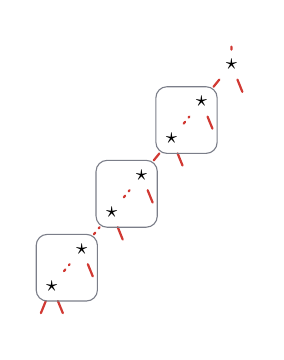
\begin{tikzpicture}[xscale=.19,yscale=.25,Centering]
            \node(0)at(0.00,-13.12){};
            \node(10)at(10.00,-5.62){};
            \node(12)at(12.00,-3.75){};
            \node(14)at(14.00,-1.88){};
            \node(2)at(2.00,-13.12){};
            \node(4)at(4.00,-11.25){};
            \node(6)at(6.00,-9.38){};
            \node(8)at(8.00,-7.50){};
            \node[NodeST](1)at(1.00,-11.25)
                {\begin{math}\Product\end{math}};
            \node[NodeST](11)at(11.00,-1.88)
                {\begin{math}\Product\end{math}};
            \node[NodeST](13)at(13.00,0.00)
                {\begin{math}\Product\end{math}};
            \node[NodeST](3)at(3.00,-9.38)
                {\begin{math}\Product\end{math}};
            \node[NodeST](5)at(5.00,-7.50)
                {\begin{math}\Product\end{math}};
            \node[NodeST](7)at(7.00,-5.62)
                {\begin{math}\Product\end{math}};
            \node[NodeST](9)at(9.00,-3.75)
                {\begin{math}\Product\end{math}};
            \draw[Edge](0)--(1);
            \draw[Edge,dotted](1)--(3);
            \draw[Edge](10)--(9);
            \draw[Edge](11)--(13);
            \draw[Edge](12)--(11);
            \draw[Edge](14)--(13);
            \draw[Edge](2)--(1);
            \draw[Edge,dotted](3)--(5);
            \draw[Edge](4)--(3);
            \draw[Edge,dotted](5)--(7);
            \draw[Edge](6)--(5);
            \draw[Edge](7)--(9);
            \draw[Edge](8)--(7);
            \draw[Edge,dotted](9)--(11);
            \node(r)at(13.00,1.41){};
            \draw[Edge](r)--(13);
            %
            \node[fit=(1)(3),rotate fit=0,inner sep=0pt,
                rounded corners,draw=Col5!80]{};
            \node[fit=(5)(7),rotate fit=0,inner sep=0pt,
                rounded corners,draw=Col5!80]{};
            \node[fit=(9)(11),rotate fit=0,inner sep=0pt,
                rounded corners,draw=Col5!80]{};
        \end{tikzpicture}
        \enspace \Rew \enspace
            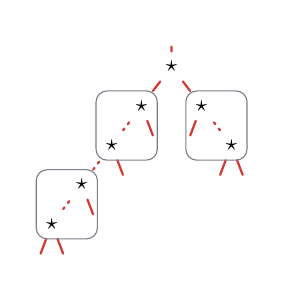
\begin{tikzpicture}[xscale=.19,yscale=.2,Centering]
            \node(0)at(0.00,-12.50){};
            \node(10)at(10.00,-5.00){};
            \node(12)at(12.00,-7.50){};
            \node(14)at(14.00,-7.50){};
            \node(2)at(2.00,-12.50){};
            \node(4)at(4.00,-10.00){};
            \node(6)at(6.00,-7.50){};
            \node(8)at(8.00,-5.00){};
            \node[NodeST](1)at(1.00,-10.00)
                {\begin{math}\Product\end{math}};
            \node[NodeST](11)at(11.00,-2.50)
                {\begin{math}\Product\end{math}};
            \node[NodeST](13)at(13.00,-5.00)
                {\begin{math}\Product\end{math}};
            \node[NodeST](3)at(3.00,-7.50)
                {\begin{math}\Product\end{math}};
            \node[NodeST](5)at(5.00,-5.00)
                {\begin{math}\Product\end{math}};
            \node[NodeST](7)at(7.00,-2.50)
                {\begin{math}\Product\end{math}};
            \node[NodeST](9)at(9.00,0.00)
                {\begin{math}\Product\end{math}};
            \draw[Edge](0)--(1);
            \draw[Edge,dotted](1)--(3);
            \draw[Edge](10)--(11);
            \draw[Edge](11)--(9);
            \draw[Edge](12)--(13);
            \draw[Edge,dotted](13)--(11);
            \draw[Edge](14)--(13);
            \draw[Edge](2)--(1);
            \draw[Edge,dotted](3)--(5);
            \draw[Edge](4)--(3);
            \draw[Edge,dotted](5)--(7);
            \draw[Edge](6)--(5);
            \draw[Edge](7)--(9);
            \draw[Edge](8)--(7);
            \node(r)at(9.00,1.88){};
            \draw[Edge](r)--(9);
            %
            \node[fit=(1)(3),rotate fit=0,inner sep=0pt,
                rounded corners,draw=Col5!80]{};
            \node[fit=(5)(7),rotate fit=0,inner sep=0pt,
                rounded corners,draw=Col5!80]{};
            \node[fit=(11)(13),rotate fit=0,inner sep=0pt,
                rounded corners,draw=Col5!80]{};
        \end{tikzpicture}
        \enspace \Rew \enspace
        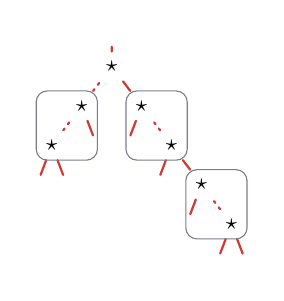
\begin{tikzpicture}[xscale=.19,yscale=.2,Centering]
            \node(0)at(0.00,-7.50){};
            \node(10)at(10.00,-10.00){};
            \node(12)at(12.00,-12.50){};
            \node(14)at(14.00,-12.50){};
            \node(2)at(2.00,-7.50){};
            \node(4)at(4.00,-5.00){};
            \node(6)at(6.00,-5.00){};
            \node(8)at(8.00,-7.50){};
            \node[NodeST](1)at(1.00,-5.00)
                {\begin{math}\Product\end{math}};
            \node[NodeST](11)at(11.00,-7.50)
                {\begin{math}\Product\end{math}};
            \node[NodeST](13)at(13.00,-10.00)
                {\begin{math}\Product\end{math}};
            \node[NodeST](3)at(3.00,-2.50)
                {\begin{math}\Product\end{math}};
            \node[NodeST](5)at(5.00,0.00)
                {\begin{math}\Product\end{math}};
            \node[NodeST](7)at(7.00,-2.50)
                {\begin{math}\Product\end{math}};
            \node[NodeST](9)at(9.00,-5.00)
                {\begin{math}\Product\end{math}};
            \draw[Edge](0)--(1);
            \draw[Edge,dotted](1)--(3);
            \draw[Edge](10)--(11);
            \draw[Edge](11)--(9);
            \draw[Edge](12)--(13);
            \draw[Edge,dotted](13)--(11);
            \draw[Edge](14)--(13);
            \draw[Edge](2)--(1);
            \draw[Edge,dotted](3)--(5);
            \draw[Edge](4)--(3);
            \draw[Edge](6)--(7);
            \draw[Edge](7)--(5);
            \draw[Edge](8)--(9);
            \draw[Edge,dotted](9)--(7);
            \node(r)at(5.00,1.88){};
            \draw[Edge](r)--(5);
            %
            \node[fit=(1)(3),rotate fit=0,inner sep=0pt,
                rounded corners,draw=Col5!80]{};
            \node[fit=(7)(9),rotate fit=0,inner sep=0pt,
                rounded corners,draw=Col5!80]{};
            \node[fit=(11)(13),rotate fit=0,inner sep=0pt,
                rounded corners,draw=Col5!80]{};
        \end{tikzpicture} \\
        \enspace \RewRT \enspace
        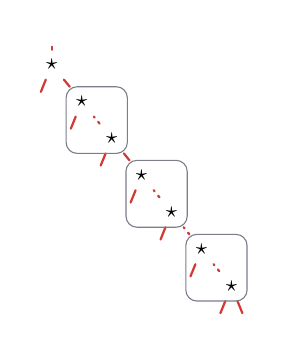
\begin{tikzpicture}[xscale=.19,yscale=.25,Centering]
            \node(0)at(0.00,-1.88){};
            \node(10)at(10.00,-11.25){};
            \node(12)at(12.00,-13.12){};
            \node(14)at(14.00,-13.12){};
            \node(2)at(2.00,-3.75){};
            \node(4)at(4.00,-5.62){};
            \node(6)at(6.00,-7.50){};
            \node(8)at(8.00,-9.38){};
            \node[NodeST](1)at(1.00,0.00)
                {\begin{math}\Product\end{math}};
            \node[NodeST](11)at(11.00,-9.38)
                {\begin{math}\Product\end{math}};
            \node[NodeST](13)at(13.00,-11.25)
                {\begin{math}\Product\end{math}};
            \node[NodeST](3)at(3.00,-1.88)
                {\begin{math}\Product\end{math}};
            \node[NodeST](5)at(5.00,-3.75)
                {\begin{math}\Product\end{math}};
            \node[NodeST](7)at(7.00,-5.62)
                {\begin{math}\Product\end{math}};
            \node[NodeST](9)at(9.00,-7.50)
                {\begin{math}\Product\end{math}};
            \draw[Edge](0)--(1);
            \draw[Edge](10)--(11);
            \draw[Edge,dotted](11)--(9);
            \draw[Edge](12)--(13);
            \draw[Edge,dotted](13)--(11);
            \draw[Edge](14)--(13);
            \draw[Edge](2)--(3);
            \draw[Edge](3)--(1);
            \draw[Edge](4)--(5);
            \draw[Edge,dotted](5)--(3);
            \draw[Edge](6)--(7);
            \draw[Edge](7)--(5);
            \draw[Edge](8)--(9);
            \draw[Edge,dotted](9)--(7);
            \node(r)at(1.00,1.41){};
            \draw[Edge](r)--(1);
            %
            \node[fit=(3)(5),rotate fit=0,inner sep=0pt,
                rounded corners,draw=Col5!80]{};
            \node[fit=(7)(9),rotate fit=0,inner sep=0pt,
                rounded corners,draw=Col5!80]{};
            \node[fit=(11)(13),rotate fit=0,inner sep=0pt,
                rounded corners,draw=Col5!80]{};
        \end{tikzpicture}
        \enspace = \enspace
        \RComb{\gamma'}
    \end{multline}
    of rewriting steps, where squared regions denotes left or right
    comb trees of degree $\gamma - 1$. Hence, we have
    $\LComb{\gamma'}\CongrCAs{\gamma}\RComb{\gamma'}$.
\end{proof}
\medbreak

Proposition~\ref{prop:division_CAs} implies the following result.
\medbreak

\begin{Theorem}\label{thm:lattice_CAs}
    The poset $\left(\CAsAll, \OrdCAs\right)$ is a lattice where
    the lower-bound and upper-bound satisfy, for any positive integers
    $\gamma$ and $\gamma'$,
    \begin{equation}
        \CAs{\gamma} \wedge \CAs{\gamma'}
        = \CAs{\gcd \left(\gamma-1, \gamma'-1\right)}
    \end{equation}
    and
    \begin{equation}
        \CAs{\gamma} \vee \CAs{\gamma'}
        = \CAs{\lcm \left(\gamma-1, \gamma'-1\right)}.
    \end{equation}
\end{Theorem}
\medbreak

%%%%%%%%%%%%%%%%%%%%%%%%%%%%%%%%%%%%%%%%%%%%%%%%%%%%%%%%%%%%%%%%%%%%%%%%
%%%%%%%%%%%%%%%%%%%%%%%%%%%%%%%%%%%%%%%%%%%%%%%%%%%%%%%%%%%%%%%%%%%%%%%%
%%%%%%%%%%%%%%%%%%%%%%%%%%%%%%%%%%%%%%%%%%%%%%%%%%%%%%%%%%%%%%%%%%%%%%%%
\section{The \texorpdfstring{$3$}{3}-comb associative operad}
\label{sec:CAs_3}
We now focus on the study of the operad $\CAs{3}$. By definition, this
operad is the quotient of $\Mag$ by the operad congruence spanned by the
relation
\begin{equation} \label{equ:rew_1}
    \begin{tikzpicture}[xscale=.22,yscale=.23,Centering]
        \node(0)at(0.00,-5.25){};
        \node(2)at(2.00,-5.25){};
        \node(4)at(4.00,-3.50){};
        \node(6)at(6.00,-1.75){};
        \node[NodeST](1)at(1.00,-3.50){\begin{math}\Product\end{math}};
        \node[NodeST](3)at(3.00,-1.75){\begin{math}\Product\end{math}};
        \node[NodeST](5)at(5.00,0.00){\begin{math}\Product\end{math}};
        \draw[Edge](0)--(1);
        \draw[Edge](1)--(3);
        \draw[Edge](2)--(1);
        \draw[Edge](3)--(5);
        \draw[Edge](4)--(3);
        \draw[Edge](6)--(5);
        \node(r)at(5.00,1.5){};
        \draw[Edge](r)--(5);
    \end{tikzpicture}
    \enspace \Rew \enspace
    \begin{tikzpicture}[xscale=.22,yscale=.23,Centering]
        \node(0)at(0.00,-1.75){};
        \node(2)at(2.00,-3.50){};
        \node(4)at(4.00,-5.25){};
        \node(6)at(6.00,-5.25){};
        \node[NodeST](1)at(1.00,0.00){\begin{math}\Product\end{math}};
        \node[NodeST](3)at(3.00,-1.75){\begin{math}\Product\end{math}};
        \node[NodeST](5)at(5.00,-3.50){\begin{math}\Product\end{math}};
        \draw[Edge](0)--(1);
        \draw[Edge](2)--(3);
        \draw[Edge](3)--(1);
        \draw[Edge](4)--(5);
        \draw[Edge](5)--(3);
        \draw[Edge](6)--(5);
        \node(r)at(1.00,1.5){};
        \draw[Edge](r)--(1);
    \end{tikzpicture}\,.
\end{equation}
This rewrite rule is compatible with the lexicographic order on prefix
words presented at the beginning of Section~\ref{sec:operad_Mag} in the
sense that the prefix word of the left member of~\eqref{equ:rew_1} is
lexicographically greater than the prefix word of the right one.
\medbreak

However, the rewrite relation $\RewContext$ induced by $\Rew$ is not
confluent. Indeed, we have
\begin{equation} \label{equ:branching_pair_CAs_3}
    \begin{tikzpicture}[xscale=.22,yscale=.22,Centering]
        \node(0)at(0.00,-7.20){};
        \node(2)at(2.00,-7.20){};
        \node(4)at(4.00,-5.40){};
        \node(6)at(6.00,-3.60){};
        \node(8)at(8.00,-1.80){};
        \node[NodeST](1)at(1.00,-5.40){\begin{math}\Product\end{math}};
        \node[NodeST](3)at(3.00,-3.60){\begin{math}\Product\end{math}};
        \node[NodeST](5)at(5.00,-1.80){\begin{math}\Product\end{math}};
        \node[NodeST](7)at(7.00,0.00){\begin{math}\Product\end{math}};
        \draw[Edge](0)--(1);
        \draw[Edge](1)--(3);
        \draw[Edge](2)--(1);
        \draw[Edge](3)--(5);
        \draw[Edge](4)--(3);
        \draw[Edge](5)--(7);
        \draw[Edge](6)--(5);
        \draw[Edge](8)--(7);
        \node(r)at(7.00,1.35){};
        \draw[Edge](r)--(7);
    \end{tikzpicture}
    \enspace \RewContext \enspace
    \begin{tikzpicture}[xscale=.22,yscale=.20,Centering]
        \node(0)at(0.00,-4.50){};
        \node(2)at(2.00,-4.50){};
        \node(4)at(4.00,-4.50){};
        \node(6)at(6.00,-6.75){};
        \node(8)at(8.00,-6.75){};
        \node[NodeST](1)at(1.00,-2.25){\begin{math}\Product\end{math}};
        \node[NodeST](3)at(3.00,0.00){\begin{math}\Product\end{math}};
        \node[NodeST](5)at(5.00,-2.25){\begin{math}\Product\end{math}};
        \node[NodeST](7)at(7.00,-4.50){\begin{math}\Product\end{math}};
        \draw[Edge](0)--(1);
        \draw[Edge](1)--(3);
        \draw[Edge](2)--(1);
        \draw[Edge](4)--(5);
        \draw[Edge](5)--(3);
        \draw[Edge](6)--(7);
        \draw[Edge](7)--(5);
        \draw[Edge](8)--(7);
        \node(r)at(3.00,1.74){};
        \draw[Edge](r)--(3);
    \end{tikzpicture}
    \qquad \mbox{and} \qquad
    \begin{tikzpicture}[xscale=.22,yscale=.22,Centering]
        \node(0)at(0.00,-7.20){};
        \node(2)at(2.00,-7.20){};
        \node(4)at(4.00,-5.40){};
        \node(6)at(6.00,-3.60){};
        \node(8)at(8.00,-1.80){};
        \node[NodeST](1)at(1.00,-5.40){\begin{math}\Product\end{math}};
        \node[NodeST](3)at(3.00,-3.60){\begin{math}\Product\end{math}};
        \node[NodeST](5)at(5.00,-1.80){\begin{math}\Product\end{math}};
        \node[NodeST](7)at(7.00,0.00){\begin{math}\Product\end{math}};
        \draw[Edge](0)--(1);
        \draw[Edge](1)--(3);
        \draw[Edge](2)--(1);
        \draw[Edge](3)--(5);
        \draw[Edge](4)--(3);
        \draw[Edge](5)--(7);
        \draw[Edge](6)--(5);
        \draw[Edge](8)--(7);
        \node(r)at(7.00,1.35){};
        \draw[Edge](r)--(7);
    \end{tikzpicture}
    \enspace \RewContext \enspace
    \begin{tikzpicture}[xscale=.22,yscale=.22,Centering]
        \node(0)at(0.00,-3.60){};
        \node(2)at(2.00,-5.40){};
        \node(4)at(4.00,-7.20){};
        \node(6)at(6.00,-7.20){};
        \node(8)at(8.00,-1.80){};
        \node[NodeST](1)at(1.00,-1.80){\begin{math}\Product\end{math}};
        \node[NodeST](3)at(3.00,-3.60){\begin{math}\Product\end{math}};
        \node[NodeST](5)at(5.00,-5.40){\begin{math}\Product\end{math}};
        \node[NodeST](7)at(7.00,0.00){\begin{math}\Product\end{math}};
        \draw[Edge](0)--(1);
        \draw[Edge](1)--(7);
        \draw[Edge](2)--(3);
        \draw[Edge](3)--(1);
        \draw[Edge](4)--(5);
        \draw[Edge](5)--(3);
        \draw[Edge](6)--(5);
        \draw[Edge](8)--(7);
        \node(r)at(7.00,1.5){};
        \draw[Edge](r)--(7);
    \end{tikzpicture}\,,
\end{equation}
and the two right members of~\eqref{equ:branching_pair_CAs_3} form a
branching pair which is not joinable.
\medbreak

In order to transform the rewrite relation induced by~\eqref{equ:rew_1}
into a convergent one, we apply the Buchberger algorithm for
operads~\cite[Section 3.7]{DK10} with respect to the lexicographic order
on prefix words. Following this algorithm, we need to put the right
members of~\eqref{equ:branching_pair_CAs_3} in relation by $\Rew$. To
respect the lexicographic property of the prefix words, this leads to
the new relation
\begin{equation} \label{equ:rew_2}
    \begin{tikzpicture}[xscale=.22,yscale=.22,Centering]
        \node(0)at(0.00,-3.60){};
        \node(2)at(2.00,-5.40){};
        \node(4)at(4.00,-7.20){};
        \node(6)at(6.00,-7.20){};
        \node(8)at(8.00,-1.80){};
        \node[NodeST](1)at(1.00,-1.80){\begin{math}\Product\end{math}};
        \node[NodeST](3)at(3.00,-3.60){\begin{math}\Product\end{math}};
        \node[NodeST](5)at(5.00,-5.40){\begin{math}\Product\end{math}};
        \node[NodeST](7)at(7.00,0.00){\begin{math}\Product\end{math}};
        \draw[Edge](0)--(1);
        \draw[Edge](1)--(7);
        \draw[Edge](2)--(3);
        \draw[Edge](3)--(1);
        \draw[Edge](4)--(5);
        \draw[Edge](5)--(3);
        \draw[Edge](6)--(5);
        \draw[Edge](8)--(7);
        \node(r)at(7.00,1.5){};
        \draw[Edge](r)--(7);
    \end{tikzpicture}
    \enspace \Rew \enspace
    \begin{tikzpicture}[xscale=.22,yscale=.20,Centering]
        \node(0)at(0.00,-4.50){};
        \node(2)at(2.00,-4.50){};
        \node(4)at(4.00,-4.50){};
        \node(6)at(6.00,-6.75){};
        \node(8)at(8.00,-6.75){};
        \node[NodeST](1)at(1.00,-2.25){\begin{math}\Product\end{math}};
        \node[NodeST](3)at(3.00,0.00){\begin{math}\Product\end{math}};
        \node[NodeST](5)at(5.00,-2.25){\begin{math}\Product\end{math}};
        \node[NodeST](7)at(7.00,-4.50){\begin{math}\Product\end{math}};
        \draw[Edge](0)--(1);
        \draw[Edge](1)--(3);
        \draw[Edge](2)--(1);
        \draw[Edge](4)--(5);
        \draw[Edge](5)--(3);
        \draw[Edge](6)--(7);
        \draw[Edge](7)--(5);
        \draw[Edge](8)--(7);
        \node(r)at(3.00,1.74){};
        \draw[Edge](r)--(3);
    \end{tikzpicture}\,.
\end{equation}
The Buchberger algorithm applied on binary trees of degrees $5$, $6$,
and $7$ provides the new relations \\
\begin{minipage}{7cm}
\begin{equation} \label{equ:rew_3}
    \begin{tikzpicture}[xscale=.23,yscale=.21,Centering]
        \node(0)at(0.00,-1.83){};
        \node(10)at(10.00,-5.50){};
        \node(2)at(2.00,-3.67){};
        \node(4)at(4.00,-7.33){};
        \node(6)at(6.00,-9.17){};
        \node(8)at(8.00,-9.17){};
        \node[NodeST](1)at(1.00,0.00){\begin{math}\Product\end{math}};
        \node[NodeST](3)at(3.00,-1.83){\begin{math}\Product\end{math}};
        \node[NodeST](5)at(5.00,-5.50){\begin{math}\Product\end{math}};
        \node[NodeST](7)at(7.00,-7.33){\begin{math}\Product\end{math}};
        \node[NodeST](9)at(9.00,-3.67){\begin{math}\Product\end{math}};
        \draw[Edge](0)--(1);
        \draw[Edge](10)--(9);
        \draw[Edge](2)--(3);
        \draw[Edge](3)--(1);
        \draw[Edge](4)--(5);
        \draw[Edge](5)--(9);
        \draw[Edge](6)--(7);
        \draw[Edge](7)--(5);
        \draw[Edge](8)--(7);
        \draw[Edge](9)--(3);
        \node(r)at(1.00,1.75){};
        \draw[Edge](r)--(1);
    \end{tikzpicture}
    \enspace \Rew \enspace
    \begin{tikzpicture}[xscale=.22,yscale=.24,Centering]
        \node(0)at(0.00,-1.83){};
        \node(10)at(10.00,-9.17){};
        \node(2)at(2.00,-3.67){};
        \node(4)at(4.00,-5.50){};
        \node(6)at(6.00,-7.33){};
        \node(8)at(8.00,-9.17){};
        \node[NodeST](1)at(1.00,0.00){\begin{math}\Product\end{math}};
        \node[NodeST](3)at(3.00,-1.83){\begin{math}\Product\end{math}};
        \node[NodeST](5)at(5.00,-3.67){\begin{math}\Product\end{math}};
        \node[NodeST](7)at(7.00,-5.50){\begin{math}\Product\end{math}};
        \node[NodeST](9)at(9.00,-7.33){\begin{math}\Product\end{math}};
        \draw[Edge](0)--(1);
        \draw[Edge](10)--(9);
        \draw[Edge](2)--(3);
        \draw[Edge](3)--(1);
        \draw[Edge](4)--(5);
        \draw[Edge](5)--(3);
        \draw[Edge](6)--(7);
        \draw[Edge](7)--(5);
        \draw[Edge](8)--(9);
        \draw[Edge](9)--(7);
        \node(r)at(1.00,1.5){};
        \draw[Edge](r)--(1);
    \end{tikzpicture}
\end{equation}
\end{minipage},
\begin{minipage}{7cm}
\begin{equation}\label{equ:rew_4}
     \begin{tikzpicture}[xscale=.2,yscale=.19,Centering]
        \node(0)at(0.00,-2.20){};
        \node(10)at(10.00,-6.60){};
        \node(2)at(2.00,-6.60){};
        \node(4)at(4.00,-8.80){};
        \node(6)at(6.00,-8.80){};
        \node(8)at(8.00,-6.60){};
        \node[NodeST](1)at(1.00,0.00){\begin{math}\Product\end{math}};
        \node[NodeST](3)at(3.00,-4.40){\begin{math}\Product\end{math}};
        \node[NodeST](5)at(5.00,-6.60){\begin{math}\Product\end{math}};
        \node[NodeST](7)at(7.00,-2.20){\begin{math}\Product\end{math}};
        \node[NodeST](9)at(9.00,-4.40){\begin{math}\Product\end{math}};
        \draw[Edge](0)--(1);
        \draw[Edge](10)--(9);
        \draw[Edge](2)--(3);
        \draw[Edge](3)--(7);
        \draw[Edge](4)--(5);
        \draw[Edge](5)--(3);
        \draw[Edge](6)--(5);
        \draw[Edge](7)--(1);
        \draw[Edge](8)--(9);
        \draw[Edge](9)--(7);
        \node(r)at(1.00,2){};
        \draw[Edge](r)--(1);
    \end{tikzpicture}
    \enspace \Rew \enspace
    \begin{tikzpicture}[xscale=.22,yscale=.24,Centering]
        \node(0)at(0.00,-1.83){};
        \node(10)at(10.00,-9.17){};
        \node(2)at(2.00,-3.67){};
        \node(4)at(4.00,-5.50){};
        \node(6)at(6.00,-7.33){};
        \node(8)at(8.00,-9.17){};
        \node[NodeST](1)at(1.00,0.00){\begin{math}\Product\end{math}};
        \node[NodeST](3)at(3.00,-1.83){\begin{math}\Product\end{math}};
        \node[NodeST](5)at(5.00,-3.67){\begin{math}\Product\end{math}};
        \node[NodeST](7)at(7.00,-5.50){\begin{math}\Product\end{math}};
        \node[NodeST](9)at(9.00,-7.33){\begin{math}\Product\end{math}};
        \draw[Edge](0)--(1);
        \draw[Edge](10)--(9);
        \draw[Edge](2)--(3);
        \draw[Edge](3)--(1);
        \draw[Edge](4)--(5);
        \draw[Edge](5)--(3);
        \draw[Edge](6)--(7);
        \draw[Edge](7)--(5);
        \draw[Edge](8)--(9);
        \draw[Edge](9)--(7);
        \node(r)at(1.00,1.75){};
        \draw[Edge](r)--(1);
    \end{tikzpicture}
\end{equation}
\end{minipage}, \\
\begin{minipage}{7cm}
\begin{equation} \label{equ:rew_5}
    \begin{tikzpicture}[xscale=.2,yscale=.2,Centering]
        \node(0)at(0.00,-2.17){};
        \node(10)at(10.00,-10.83){};
        \node(12)at(12.00,-10.83){};
        \node(2)at(2.00,-4.33){};
        \node(4)at(4.00,-8.67){};
        \node(6)at(6.00,-8.67){};
        \node(8)at(8.00,-8.67){};
        \node[NodeST](1)at(1.00,0.00){\begin{math}\Product\end{math}};
        \node[NodeST](11)at(11.00,-8.67)
            {\begin{math}\Product\end{math}};
        \node[NodeST](3)at(3.00,-2.17){\begin{math}\Product\end{math}};
        \node[NodeST](5)at(5.00,-6.50){\begin{math}\Product\end{math}};
        \node[NodeST](7)at(7.00,-4.33){\begin{math}\Product\end{math}};
        \node[NodeST](9)at(9.00,-6.50){\begin{math}\Product\end{math}};
        \draw[Edge](0)--(1);
        \draw[Edge](10)--(11);
        \draw[Edge](11)--(9);
        \draw[Edge](12)--(11);
        \draw[Edge](2)--(3);
        \draw[Edge](3)--(1);
        \draw[Edge](4)--(5);
        \draw[Edge](5)--(7);
        \draw[Edge](6)--(5);
        \draw[Edge](7)--(3);
        \draw[Edge](8)--(9);
        \draw[Edge](9)--(7);
        \node(r)at(1.00,1.75){};
        \draw[Edge](r)--(1);
    \end{tikzpicture}
    \Rew
    \begin{tikzpicture}[xscale=.21,yscale=.22,Centering]
        \node(0)at(0.00,-1.86){};
        \node(10)at(10.00,-11.14){};
        \node(12)at(12.00,-9.29){};
        \node(2)at(2.00,-3.71){};
        \node(4)at(4.00,-5.57){};
        \node(6)at(6.00,-7.43){};
        \node(8)at(8.00,-11.14){};
        \node[NodeST](1)at(1.00,0.00){\begin{math}\Product\end{math}};
        \node[NodeST](11)at(11.00,-7.43)
            {\begin{math}\Product\end{math}};
        \node[NodeST](3)at(3.00,-1.86){\begin{math}\Product\end{math}};
        \node[NodeST](5)at(5.00,-3.71){\begin{math}\Product\end{math}};
        \node[NodeST](7)at(7.00,-5.57){\begin{math}\Product\end{math}};
        \node[NodeST](9)at(9.00,-9.29){\begin{math}\Product\end{math}};
        \draw[Edge](0)--(1);
        \draw[Edge](10)--(9);
        \draw[Edge](11)--(7);
        \draw[Edge](12)--(11);
        \draw[Edge](2)--(3);
        \draw[Edge](3)--(1);
        \draw[Edge](4)--(5);
        \draw[Edge](5)--(3);
        \draw[Edge](6)--(7);
        \draw[Edge](7)--(5);
        \draw[Edge](8)--(9);
        \draw[Edge](9)--(11);
        \node(r)at(1.00,1.75){};
        \draw[Edge](r)--(1);
    \end{tikzpicture}
\end{equation}
\end{minipage},
\begin{minipage}{7cm}
\begin{equation} \label{equ:rew_6}
    \begin{tikzpicture}[xscale=.21,yscale=.21,Centering]
        \node(0)at(0.00,-2.17){};
        \node(10)at(10.00,-10.83){};
        \node(12)at(12.00,-10.83){};
        \node(2)at(2.00,-6.50){};
        \node(4)at(4.00,-6.50){};
        \node(6)at(6.00,-6.50){};
        \node(8)at(8.00,-8.67){};
        \node[NodeST](1)at(1.00,0.00){\begin{math}\Product\end{math}};
        \node[NodeST](11)at(11.00,-8.67)
            {\begin{math}\Product\end{math}};
        \node[NodeST](3)at(3.00,-4.33){\begin{math}\Product\end{math}};
        \node[NodeST](5)at(5.00,-2.17){\begin{math}\Product\end{math}};
        \node[NodeST](7)at(7.00,-4.33){\begin{math}\Product\end{math}};
        \node[NodeST](9)at(9.00,-6.50){\begin{math}\Product\end{math}};
        \draw[Edge](0)--(1);
        \draw[Edge](10)--(11);
        \draw[Edge](11)--(9);
        \draw[Edge](12)--(11);
        \draw[Edge](2)--(3);
        \draw[Edge](3)--(5);
        \draw[Edge](4)--(3);
        \draw[Edge](5)--(1);
        \draw[Edge](6)--(7);
        \draw[Edge](7)--(5);
        \draw[Edge](8)--(9);
        \draw[Edge](9)--(7);
        \node(r)at(1.00,1.75){};
        \draw[Edge](r)--(1);
    \end{tikzpicture}
    \Rew
    \begin{tikzpicture}[xscale=.22,yscale=.21,Centering]
        \node(0)at(0.00,-2.17){};
        \node(10)at(10.00,-10.83){};
        \node(12)at(12.00,-10.83){};
        \node(2)at(2.00,-4.33){};
        \node(4)at(4.00,-6.50){};
        \node(6)at(6.00,-10.83){};
        \node(8)at(8.00,-10.83){};
        \node[NodeST](1)at(1.00,0.00){\begin{math}\Product\end{math}};
        \node[NodeST](11)at(11.00,-8.67)
            {\begin{math}\Product\end{math}};
        \node[NodeST](3)at(3.00,-2.17){\begin{math}\Product\end{math}};
        \node[NodeST](5)at(5.00,-4.33){\begin{math}\Product\end{math}};
        \node[NodeST](7)at(7.00,-8.67){\begin{math}\Product\end{math}};
        \node[NodeST](9)at(9.00,-6.50){\begin{math}\Product\end{math}};
        \draw[Edge](0)--(1);
        \draw[Edge](10)--(11);
        \draw[Edge](11)--(9);
        \draw[Edge](12)--(11);
        \draw[Edge](2)--(3);
        \draw[Edge](3)--(1);
        \draw[Edge](4)--(5);
        \draw[Edge](5)--(3);
        \draw[Edge](6)--(7);
        \draw[Edge](7)--(9);
        \draw[Edge](8)--(7);
        \draw[Edge](9)--(5);
        \node(r)at(1.00,1.75){};
        \draw[Edge](r)--(1);
    \end{tikzpicture}\hspace{-8pt}
\end{equation}
\end{minipage}, \\
\begin{minipage}{7cm}
\begin{equation} \label{equ:rew_7}
    \begin{tikzpicture}[xscale=.19,yscale=.17,Centering]
        \node(0)at(0.00,-5.20){};
        \node(10)at(10.00,-7.80){};
        \node(12)at(12.00,-7.80){};
        \node(2)at(2.00,-10.40){};
        \node(4)at(4.00,-10.40){};
        \node(6)at(6.00,-7.80){};
        \node(8)at(8.00,-5.20){};
        \node[NodeST](1)at(1.00,-2.60){\begin{math}\Product\end{math}};
        \node[NodeST](11)at(11.00,-5.20)
            {\begin{math}\Product\end{math}};
        \node[NodeST](3)at(3.00,-7.80){\begin{math}\Product\end{math}};
        \node[NodeST](5)at(5.00,-5.20){\begin{math}\Product\end{math}};
        \node[NodeST](7)at(7.00,0.00){\begin{math}\Product\end{math}};
        \node[NodeST](9)at(9.00,-2.60){\begin{math}\Product\end{math}};
        \draw[Edge](0)--(1);
        \draw[Edge](1)--(7);
        \draw[Edge](10)--(11);
        \draw[Edge](11)--(9);
        \draw[Edge](12)--(11);
        \draw[Edge](2)--(3);
        \draw[Edge](3)--(5);
        \draw[Edge](4)--(3);
        \draw[Edge](5)--(1);
        \draw[Edge](6)--(5);
        \draw[Edge](8)--(9);
        \draw[Edge](9)--(7);
        \node(r)at(7.00,2){};
        \draw[Edge](r)--(7);
    \end{tikzpicture}
    \enspace \Rew \enspace
        \begin{tikzpicture}[xscale=.2,yscale=.19,Centering]
        \node(0)at(0.00,-4.33){};
        \node(10)at(10.00,-10.83){};
        \node(12)at(12.00,-10.83){};
        \node(2)at(2.00,-4.33){};
        \node(4)at(4.00,-4.33){};
        \node(6)at(6.00,-6.50){};
        \node(8)at(8.00,-8.67){};
        \node[NodeST](1)at(1.00,-2.17){\begin{math}\Product\end{math}};
        \node[NodeST](11)at(11.00,-8.67)
            {\begin{math}\Product\end{math}};
        \node[NodeST](3)at(3.00,0.00){\begin{math}\Product\end{math}};
        \node[NodeST](5)at(5.00,-2.17){\begin{math}\Product\end{math}};
        \node[NodeST](7)at(7.00,-4.33){\begin{math}\Product\end{math}};
        \node[NodeST](9)at(9.00,-6.50){\begin{math}\Product\end{math}};
        \draw[Edge](0)--(1);
        \draw[Edge](1)--(3);
        \draw[Edge](10)--(11);
        \draw[Edge](11)--(9);
        \draw[Edge](12)--(11);
        \draw[Edge](2)--(1);
        \draw[Edge](4)--(5);
        \draw[Edge](5)--(3);
        \draw[Edge](6)--(7);
        \draw[Edge](7)--(5);
        \draw[Edge](8)--(9);
        \draw[Edge](9)--(7);
        \node(r)at(3.00,1.75){};
        \draw[Edge](r)--(3);
    \end{tikzpicture}\hspace{-10pt}
\end{equation}
\end{minipage},
\begin{minipage}{7cm}
\begin{equation} \label{equ:rew_8}
    \begin{tikzpicture}[xscale=.2,yscale=.19,Centering]
        \node(0)at(0.00,-2.14){};
        \node(10)at(10.00,-12.86){};
        \node(12)at(12.00,-12.86){};
        \node(14)at(14.00,-12.86){};
        \node(2)at(2.00,-4.29){};
        \node(4)at(4.00,-6.43){};
        \node(6)at(6.00,-8.57){};
        \node(8)at(8.00,-12.86){};
        \node[NodeST](1)at(1.00,0.00){\begin{math}\Product\end{math}};
        \node[NodeST](11)at(11.00,-8.57)
            {\begin{math}\Product\end{math}};
        \node[NodeST](13)at(13.00,-10.71)
            {\begin{math}\Product\end{math}};
        \node[NodeST](3)at(3.00,-2.14){\begin{math}\Product\end{math}};
        \node[NodeST](5)at(5.00,-4.29){\begin{math}\Product\end{math}};
        \node[NodeST](7)at(7.00,-6.43){\begin{math}\Product\end{math}};
        \node[NodeST](9)at(9.00,-10.71){\begin{math}\Product\end{math}};
        \draw[Edge](0)--(1);
        \draw[Edge](10)--(9);
        \draw[Edge](11)--(7);
        \draw[Edge](12)--(13);
        \draw[Edge](13)--(11);
        \draw[Edge](14)--(13);
        \draw[Edge](2)--(3);
        \draw[Edge](3)--(1);
        \draw[Edge](4)--(5);
        \draw[Edge](5)--(3);
        \draw[Edge](6)--(7);
        \draw[Edge](7)--(5);
        \draw[Edge](8)--(9);
        \draw[Edge](9)--(11);
        \node(r)at(1.00,2){};
        \draw[Edge](r)--(1);
    \end{tikzpicture}
    \hspace{-10pt}\Rew
    \begin{tikzpicture}[xscale=.22,yscale=.2,Centering]
        \node(0)at(0.00,-1.88){};
        \node(10)at(10.00,-13.12){};
        \node(12)at(12.00,-13.12){};
        \node(14)at(14.00,-11.25){};
        \node(2)at(2.00,-3.75){};
        \node(4)at(4.00,-5.62){};
        \node(6)at(6.00,-7.50){};
        \node(8)at(8.00,-9.38){};
        \node[NodeST](1)at(1.00,0.00){\begin{math}\Product\end{math}};
        \node[NodeST](11)at(11.00,-11.25)
            {\begin{math}\Product\end{math}};
        \node[NodeST](13)at(13.00,-9.38)
            {\begin{math}\Product\end{math}};
        \node[NodeST](3)at(3.00,-1.88){\begin{math}\Product\end{math}};
        \node[NodeST](5)at(5.00,-3.75){\begin{math}\Product\end{math}};
        \node[NodeST](7)at(7.00,-5.62){\begin{math}\Product\end{math}};
        \node[NodeST](9)at(9.00,-7.50){\begin{math}\Product\end{math}};
        \draw[Edge](0)--(1);
        \draw[Edge](10)--(11);
        \draw[Edge](11)--(13);
        \draw[Edge](12)--(11);
        \draw[Edge](13)--(9);
        \draw[Edge](14)--(13);
        \draw[Edge](2)--(3);
        \draw[Edge](3)--(1);
        \draw[Edge](4)--(5);
        \draw[Edge](5)--(3);
        \draw[Edge](6)--(7);
        \draw[Edge](7)--(5);
        \draw[Edge](8)--(9);
        \draw[Edge](9)--(7);
        \node(r)at(1.00,2){};
        \draw[Edge](r)--(1);
    \end{tikzpicture}\hspace{-20pt}
\end{equation}
\end{minipage}, \\
\begin{minipage}{7cm}
\begin{equation} \label{equ:rew_9}
    \begin{tikzpicture}[xscale=0.18,yscale=.2,Centering]
        \node(0)at(0.00,-2.14){};
        \node(10)at(10.00,-12.86){};
        \node(12)at(12.00,-12.86){};
        \node(14)at(14.00,-10.71){};
        \node(2)at(2.00,-4.29){};
        \node(4)at(4.00,-6.43){};
        \node(6)at(6.00,-10.71){};
        \node(8)at(8.00,-10.71){};
        \node[NodeST](1)at(1.00,0.00){\begin{math}\Product\end{math}};
        \node[NodeST](11)at(11.00,-10.71)
            {\begin{math}\Product\end{math}};
        \node[NodeST](13)at(13.00,-8.57)
            {\begin{math}\Product\end{math}};
        \node[NodeST](3)at(3.00,-2.14){\begin{math}\Product\end{math}};
        \node[NodeST](5)at(5.00,-4.29){\begin{math}\Product\end{math}};
        \node[NodeST](7)at(7.00,-8.57){\begin{math}\Product\end{math}};
        \node[NodeST](9)at(9.00,-6.43){\begin{math}\Product\end{math}};
        \draw[Edge](0)--(1);
        \draw[Edge](10)--(11);
        \draw[Edge](11)--(13);
        \draw[Edge](12)--(11);
        \draw[Edge](13)--(9);
        \draw[Edge](14)--(13);
        \draw[Edge](2)--(3);
        \draw[Edge](3)--(1);
        \draw[Edge](4)--(5);
        \draw[Edge](5)--(3);
        \draw[Edge](6)--(7);
        \draw[Edge](7)--(9);
        \draw[Edge](8)--(7);
        \draw[Edge](9)--(5);
        \node(r)at(1.00,2){};
        \draw[Edge](r)--(1);
    \end{tikzpicture}
    \hspace{-5pt} \Rew \hspace{-5pt}
    \begin{tikzpicture}[xscale=.22,yscale=.22,Centering]
        \node(0)at(0.00,-1.88){};
        \node(10)at(10.00,-11.25){};
        \node(12)at(12.00,-13.12){};
        \node(14)at(14.00,-13.12){};
        \node(2)at(2.00,-3.75){};
        \node(4)at(4.00,-5.62){};
        \node(6)at(6.00,-7.50){};
        \node(8)at(8.00,-9.38){};
        \node[NodeST](1)at(1.00,0.00){\begin{math}\Product\end{math}};
        \node[NodeST](11)at(11.00,-9.38)
            {\begin{math}\Product\end{math}};
        \node[NodeST](13)at(13.00,-11.25)
            {\begin{math}\Product\end{math}};
        \node[NodeST](3)at(3.00,-1.88){\begin{math}\Product\end{math}};
        \node[NodeST](5)at(5.00,-3.75){\begin{math}\Product\end{math}};
        \node[NodeST](7)at(7.00,-5.62){\begin{math}\Product\end{math}};
        \node[NodeST](9)at(9.00,-7.50){\begin{math}\Product\end{math}};
        \draw[Edge](0)--(1);
        \draw[Edge](10)--(11);
        \draw[Edge](11)--(9);
        \draw[Edge](12)--(13);
        \draw[Edge](13)--(11);
        \draw[Edge](14)--(13);
        \draw[Edge](2)--(3);
        \draw[Edge](3)--(1);
        \draw[Edge](4)--(5);
        \draw[Edge](5)--(3);
        \draw[Edge](6)--(7);
        \draw[Edge](7)--(5);
        \draw[Edge](8)--(9);
        \draw[Edge](9)--(7);
        \node(r)at(1.00,1.5){};
        \draw[Edge](r)--(1);
    \end{tikzpicture}\hspace{-25pt}
\end{equation}
\end{minipage},
\begin{minipage}{7cm}
\begin{equation} \label{equ:rew_10}
    \hspace{-2pt}\begin{tikzpicture}[xscale=.2,yscale=.17,Centering]
        \node(0)at(0.00,-5.00){};
        \node(10)at(10.00,-12.50){};
        \node(12)at(12.00,-12.50){};
        \node(14)at(14.00,-12.50){};
        \node(2)at(2.00,-5.00){};
        \node(4)at(4.00,-5.00){};
        \node(6)at(6.00,-7.50){};
        \node(8)at(8.00,-12.50){};
        \node[NodeST](1)at(1.00,-2.50){\begin{math}\Product\end{math}};
        \node[NodeST](11)at(11.00,-7.50)
            {\begin{math}\Product\end{math}};
        \node[NodeST](13)at(13.00,-10.00)
            {\begin{math}\Product\end{math}};
        \node[NodeST](3)at(3.00,0.00){\begin{math}\Product\end{math}};
        \node[NodeST](5)at(5.00,-2.50){\begin{math}\Product\end{math}};
        \node[NodeST](7)at(7.00,-5.00){\begin{math}\Product\end{math}};
        \node[NodeST](9)at(9.00,-10.00){\begin{math}\Product\end{math}};
        \draw[Edge](0)--(1);
        \draw[Edge](1)--(3);
        \draw[Edge](10)--(9);
        \draw[Edge](11)--(7);
        \draw[Edge](12)--(13);
        \draw[Edge](13)--(11);
        \draw[Edge](14)--(13);
        \draw[Edge](2)--(1);
        \draw[Edge](4)--(5);
        \draw[Edge](5)--(3);
        \draw[Edge](6)--(7);
        \draw[Edge](7)--(5);
        \draw[Edge](8)--(9);
        \draw[Edge](9)--(11);
        \node(r)at(3.00,2){};
        \draw[Edge](r)--(3);
    \end{tikzpicture}
    \hspace{-10pt} \Rew \hspace{5pt}
    \begin{tikzpicture}[xscale=.21,yscale=.2,Centering]
        \node(0)at(0.00,-4.29){};
        \node(10)at(10.00,-12.86){};
        \node(12)at(12.00,-12.86){};
        \node(14)at(14.00,-10.71){};
        \node(2)at(2.00,-4.29){};
        \node(4)at(4.00,-4.29){};
        \node(6)at(6.00,-6.43){};
        \node(8)at(8.00,-8.57){};
        \node[NodeST](1)at(1.00,-2.14){\begin{math}\Product\end{math}};
        \node[NodeST](11)at(11.00,-10.71)
            {\begin{math}\Product\end{math}};
        \node[NodeST](13)at(13.00,-8.57)
            {\begin{math}\Product\end{math}};
        \node[NodeST](3)at(3.00,0.00){\begin{math}\Product\end{math}};
        \node[NodeST](5)at(5.00,-2.14){\begin{math}\Product\end{math}};
        \node[NodeST](7)at(7.00,-4.29){\begin{math}\Product\end{math}};
        \node[NodeST](9)at(9.00,-6.43){\begin{math}\Product\end{math}};
        \draw[Edge](0)--(1);
        \draw[Edge](1)--(3);
        \draw[Edge](10)--(11);
        \draw[Edge](11)--(13);
        \draw[Edge](12)--(11);
        \draw[Edge](13)--(9);
        \draw[Edge](14)--(13);
        \draw[Edge](2)--(1);
        \draw[Edge](4)--(5);
        \draw[Edge](5)--(3);
        \draw[Edge](6)--(7);
        \draw[Edge](7)--(5);
        \draw[Edge](8)--(9);
        \draw[Edge](9)--(7);
        \node(r)at(3.00,2){};
        \draw[Edge](r)--(3);
    \end{tikzpicture} \hspace{-25pt}
\end{equation}
\end{minipage}, \\
\begin{minipage}{8.8cm}
\begin{equation} \label{equ:rew_11}
    \begin{tikzpicture}[xscale=.22,yscale=.18,Centering]
        \node(0)at(0.00,-5.00){};
        \node(10)at(10.00,-10.00){};
        \node(12)at(12.00,-12.50){};
        \node(14)at(14.00,-12.50){};
        \node(2)at(2.00,-7.50){};
        \node(4)at(4.00,-7.50){};
        \node(6)at(6.00,-5.00){};
        \node(8)at(8.00,-7.50){};
        \node[NodeST](1)at(1.00,-2.50){\begin{math}\Product\end{math}};
        \node[NodeST](11)at(11.00,-7.50)
            {\begin{math}\Product\end{math}};
        \node[NodeST](13)at(13.00,-10.00)
            {\begin{math}\Product\end{math}};
        \node[NodeST](3)at(3.00,-5.00){\begin{math}\Product\end{math}};
        \node[NodeST](5)at(5.00,0.00){\begin{math}\Product\end{math}};
        \node[NodeST](7)at(7.00,-2.50){\begin{math}\Product\end{math}};
        \node[NodeST](9)at(9.00,-5.00){\begin{math}\Product\end{math}};
        \draw[Edge](0)--(1);
        \draw[Edge](1)--(5);
        \draw[Edge](10)--(11);
        \draw[Edge](11)--(9);
        \draw[Edge](12)--(13);
        \draw[Edge](13)--(11);
        \draw[Edge](14)--(13);
        \draw[Edge](2)--(3);
        \draw[Edge](3)--(1);
        \draw[Edge](4)--(3);
        \draw[Edge](6)--(7);
        \draw[Edge](7)--(5);
        \draw[Edge](8)--(9);
        \draw[Edge](9)--(7);
        \node(r)at(5.00,2){};
        \draw[Edge](r)--(5);
    \end{tikzpicture}
    \enspace \Rew \enspace
    \begin{tikzpicture}[xscale=.21,yscale=.19,Centering]
        \node(0)at(0.00,-4.29){};
        \node(10)at(10.00,-12.86){};
        \node(12)at(12.00,-12.86){};
        \node(14)at(14.00,-10.71){};
        \node(2)at(2.00,-4.29){};
        \node(4)at(4.00,-4.29){};
        \node(6)at(6.00,-6.43){};
        \node(8)at(8.00,-8.57){};
        \node[NodeST](1)at(1.00,-2.14){\begin{math}\Product\end{math}};
        \node[NodeST](11)at(11.00,-10.71)
            {\begin{math}\Product\end{math}};
        \node[NodeST](13)at(13.00,-8.57)
            {\begin{math}\Product\end{math}};
        \node[NodeST](3)at(3.00,0.00){\begin{math}\Product\end{math}};
        \node[NodeST](5)at(5.00,-2.14){\begin{math}\Product\end{math}};
        \node[NodeST](7)at(7.00,-4.29){\begin{math}\Product\end{math}};
        \node[NodeST](9)at(9.00,-6.43){\begin{math}\Product\end{math}};
        \draw[Edge](0)--(1);
        \draw[Edge](1)--(3);
        \draw[Edge](10)--(11);
        \draw[Edge](11)--(13);
        \draw[Edge](12)--(11);
        \draw[Edge](13)--(9);
        \draw[Edge](14)--(13);
        \draw[Edge](2)--(1);
        \draw[Edge](4)--(5);
        \draw[Edge](5)--(3);
        \draw[Edge](6)--(7);
        \draw[Edge](7)--(5);
        \draw[Edge](8)--(9);
        \draw[Edge](9)--(7);
        \node(r)at(3.00,2){};
        \draw[Edge](r)--(3);
    \end{tikzpicture}
\end{equation}
\end{minipage}.


\noindent
We claim that the rewrite relation $\RewContext$ induced by
rewrite rule $\Rew$ satisfying~\eqref{equ:rew_1}, \eqref{equ:rew_2},
\eqref{equ:rew_3}---\eqref{equ:rew_11} is convergent. First, for every
relation $\Tfr \Rew \Tfr'$, we have
$\PrefixWord(\Tfr) > \PrefixWord(\Tfr')$. Therefore, by
Lemma~\ref{lem:prefix_word_termination}, $\RewContext$ is terminating.
Moreover, the greatest degree of a tree appearing in $\Rew$ is~$7$ so
that, from Lemma~\ref{lem:degree_confluence}, to show that $\RewContext$
is convergent, it is enough to prove that each tree of degree at most
$13$ admits exactly one normal form. Equivalently, this amounts to
show that the number of normal forms of trees of arity $n$ is equal
to $\#\CAs{3}(n)$. By computer exploration, we get the same sequence
\begin{equation} \label{equ:dimensions_CAs_3}
    1, 1, 2, 4, 8, 14, 20, 19, 16, 14, 14, 15, 16, 17
\end{equation}
for $\#\CAs{3}(n)$ and for the numbers of normal forms of arity $n$,
when $ 1 \leq n \leq 14$. Hence, we get our following main result.
\medbreak

\begin{Theorem} \label{thm:convergent_rewrite_rule_CAs_3}
    The rewrite rule $\Rew$ satisfying~\eqref{equ:rew_1},
    \eqref{equ:rew_2}, \eqref{equ:rew_3}---\eqref{equ:rew_11} is a
    convergent orientation of the congruence $\CongrCAs{3}$
    of~$\CAs{3}$.
\end{Theorem}
\medbreak

The rewrite rule $\Rew$ has, arity by arity, the cardinalities
\begin{equation}
    0, 0, 0, 1, 1, 2, 3, 4, 0, \dots~.
\end{equation}
We obtain from Theorem~\ref{thm:convergent_rewrite_rule_CAs_3} also
the following consequences.
\medbreak

\begin{Proposition} \label{prop:PBW_basis_CAs_3}
    The set of the trees avoiding as subtrees the ones appearing as
    left members of $\Rew$ is a Poincaré-Birkhoff-Witt basis
    of~$\CAs{3}$.
\end{Proposition}
\medbreak

From Proposition~\ref{prop:PBW_basis_CAs_3}, and by using a result
of~\cite{Gir18} describing a system of equations for the generating
series of syntax trees avoiding some sets of subtrees, we obtain the
following result.
\medbreak

\begin{Proposition} \label{prop:Hilbert_series_CAs_3}
    The Hilbert series of $\CAs{3}$ is
    \begin{equation} \label{equ:Hilbert_series_CAs_3}
        \HilbertSeries_{\CAs{3}}(t) = \frac{t}{(1 - t)^2}
        \left(1 - t + t^2 + t^3 + 2t^4 + 2t^5 - 7t^7 - 2t^8 + t^9 +
        2t^{10} + t^{11}\right).
    \end{equation}
\end{Proposition}
\medbreak

For $n \leq 10$, the dimensions of $\CAs{3}(n)$ are provided by
Sequence~\eqref{equ:dimensions_CAs_3} and for all $n \geq 11$, the
Taylor expansion of~\eqref{equ:Hilbert_series_CAs_3} shows that
$\# \CAs{3}(n) = n + 3$.
\medbreak

%%%%%%%%%%%%%%%%%%%%%%%%%%%%%%%%%%%%%%%%%%%%%%%%%%%%%%%%%%%%%%%%%%%%%%%%
%%%%%%%%%%%%%%%%%%%%%%%%%%%%%%%%%%%%%%%%%%%%%%%%%%%%%%%%%%%%%%%%%%%%%%%%
%%%%%%%%%%%%%%%%%%%%%%%%%%%%%%%%%%%%%%%%%%%%%%%%%%%%%%%%%%%%%%%%%%%%%%%%
\section*{Perspectives}
Our first axis of perspectives consists in collecting properties about
the operads $\CAs{d}$. A natural question consists in finding all the
morphisms between the operads $\CAs{d}$. Some surjective morphisms are
described by Proposition~\ref{prop:quotients_CAs_d} and we can hope to a
full description of these, as well as some possible injections.
Moreover, we can try to obtain a convergent orientation of
$\CongrCAs{d}$ and general expressions of the Hilbert series of
$\CAs{d}$ when $d \geq 4$. By computer exploration, we have the sequence
\begin{equation}
    1, 1, 2, 5, 13, 35, 96, 264, 724, 1973, 5355, 14390
\end{equation}
for the first dimensions for $\CAs{4}$. By applying the Buchberger
algorithm on trees of degrees until $10$, we obtain that a convergent
orientation of $\CongrCAs{4}$ has, arity by arity, the sequence
\begin{math}
    0, 0, 0, 0, 1, 1, 0, 3, 4, 5, 18, 22
\end{math}
for its first cardinalities. Moreover, for $\CAs{5}$, we get the
sequence
\begin{equation}
    1, 1, 2, 5, 14, 41, 124, 384, 1210, 3861, 12440
\end{equation}
of dimensions and the first cardinalities
\begin{math}
    0, 0, 0, 0, 0, 1, 1, 0, 0, 4, 5
\end{math}
for any convergent orientation of $\CongrCAs{5}$. Finally, for
$\CAs{6}$, we get the sequence
\begin{equation}
    1, 1, 2, 5, 14, 42, 131, 420, 1375, 4576, 15431
\end{equation}
of dimensions and the first cardinalities
\begin{math}
    0, 0, 0, 0, 0, 0, 1, 1, 0, 0, 0
\end{math}
for any convergent orientation of $\CongrCAs{6}$. We can notice that
only $\CAs{3}$ seems to have oscillating first dimensions.
\medbreak

A second axis concerns a complete understanding of $\CAs{3}$. We can
try to construct an explicit basis of this operad.
Proposition~\ref{prop:PBW_basis_CAs_3} describes a basis in terms of
trees avoiding some patterns but, we can hope to find a simpler
description. This includes the description of a family of combinatorial
objects forming a basis of $\CAs{3}$ and an adequate definition of a
partial composition map $\circ_i$ on these. Moreover, a natural
question is to explore the suboperads $\CAs{3}$ in the category of
vector spaces.
\medbreak

In a last axis, we can consider further generalizations of $\As$ being
quotients of $\Mag$ by congruences defined by identifying certain binary
trees of a same fixed degree. A possible question is, as presented in
the introduction, to investigate if combinatorial properties of the
trees belonging to a same equivalence class imply algebraic properties
on the obtained operads.
\medbreak

%%%%%%%%%%%%%%%%%%%%%%%%%%%%%%%%%%%%%%%%%%%%%%%%%%%%%%%%%%%%%%%%%%%%%%%%
%%%%%%%%%%%%%%%%%%%%%%%%%%%%%%%%%%%%%%%%%%%%%%%%%%%%%%%%%%%%%%%%%%%%%%%%
%%%%%%%%%%%%%%%%%%%%%%%%%%%%%%%%%%%%%%%%%%%%%%%%%%%%%%%%%%%%%%%%%%%%%%%%
\bibliographystyle{alpha}
\bibliography{Bibliography}

\end{document}
